%%%%%%%%%%%%%%%%%%%%%%%%%%%%%%%%%%%%%%%%%
% Journal Article
% LaTeX Template
% Version 1.4 (15/5/16)
%
% This template has been downloaded from:
% http://www.LaTeXTemplates.com
%
% Original author:
% Frits Wenneker (http://www.howtotex.com) with extensive modifications by
% Vel (vel@LaTeXTemplates.com)
%
% License:
% CC BY-NC-SA 3.0 (http://creativecommons.org/licenses/by-nc-sa/3.0/)
%
%%%%%%%%%%%%%%%%%%%%%%%%%%%%%%%%%%%%%%%%%

%----------------------------------------------------------------------------------------
%	PACKAGES AND OTHER DOCUMENT CONFIGURATIONS
%----------------------------------------------------------------------------------------

\documentclass[twoside,twocolumn]{article}

\usepackage{blindtext} % Package to generate dummy text throughout this template 

\usepackage[sc]{mathpazo} % Use the Palatino font
\usepackage[T1]{fontenc} % Use 8-bit encoding that has 256 glyphs
\linespread{1.05} % Line spacing - Palatino needs more space between lines
\usepackage{microtype} % Slightly tweak font spacing for aesthetics

\usepackage[english]{babel} % Language hyphenation and typographical rules

\usepackage[hmarginratio=1:1,top=32mm,columnsep=20pt]{geometry} % Document margins
\usepackage[hang, small,labelfont=bf,up,textfont=it,up]{caption} % Custom captions under/above floats in tables or figures
\usepackage{booktabs} % Horizontal rules in tables

\usepackage{lettrine} % The lettrine is the first enlarged letter at the beginning of the text

\usepackage{enumitem} % Customized lists
\setlist[itemize]{noitemsep} % Make itemize lists more compact

\usepackage{abstract} % Allows abstract customization
\renewcommand{\abstractnamefont}{\normalfont\bfseries} % Set the "Abstract" text to bold
\renewcommand{\abstracttextfont}{\normalfont\small\itshape} % Set the abstract itself to small italic text

\usepackage{titlesec} % Allows customization of titles
\renewcommand\thesection{\Roman{section}} % Roman numerals for the sections
\renewcommand\thesubsection{\roman{subsection}} % roman numerals for subsections
\titleformat{\section}[block]{\large\scshape\centering}{\thesection.}{1em}{} % Change the look of the section titles
\titleformat{\subsection}[block]{\large}{\thesubsection.}{1em}{} % Change the look of the section titles

\usepackage{fancyhdr} % Headers and footers
\pagestyle{fancy} % All pages have headers and footers
\fancyhead{} % Blank out the default header
\fancyfoot{} % Blank out the default footer
\fancyhead[C]{Running title $\bullet$ May 2016 $\bullet$ Vol. XXI, No. 1} % Custom header text
\fancyfoot[RO,LE]{\thepage} % Custom footer text

\usepackage{titling} % Customizing the title section

\usepackage{hyperref} % For hyperlinks in the PDF

%----------------------------------------------------------------------------------------
%	TITLE SECTION
%----------------------------------------------------------------------------------------

\setlength{\droptitle}{-4\baselineskip} % Move the title up

\pretitle{\begin{center}\Huge\bfseries} % Article title formatting
\posttitle{\end{center}} % Article title closing formatting
\title{Android Code Smells} % Article title
\author{
	% Firts Author
	\textsc{Suelen G. Carvalho}\thanks{A thank you or further information} \\[1ex]
	\normalsize University of S�o Paulo \\
	\normalsize \href{mailto:suelengc@ime.usp.br}{suelengc@ime.usp.br}
	\and % Second Author
	\textsc{Marco A. Gerosa}\thanks{Corresponding author} \\[1ex]
	\normalsize University of S�o Paulo \\
	\normalsize \href{mailto:gerosa@ime.usp.br}{gerosa@ime.usp.br}
	\and % Third Author
	\textsc{Maur�cio Aniche}\thanks{Corresponding author} \\[1ex]
	\normalsize Delft University of Technology \\
	\normalsize \href{mailto:m.f.aniche@tudelft.nl}{m.f.aniche@tudelft.nl}
}
\date{\today} % Leave empty to omit a date

%----------------------------------------------------------------------------------------
%	ABSTRACT
%----------------------------------------------------------------------------------------

\renewcommand{\maketitlehookd}{
	\begin{abstract}
	Android is the most widely used mobile operating system with 83\% of the world market and more than 2 million applications available in the official store. Android applications have been made complex software projects that need to be quickly developed and regularly evolved to meet the requirements of users. This context can lead to bad code design choices, known as code smells, that can become anomalies that degrade project quality, making it difficult to maintain. Consequently, software developers need to identify problematic code snippets in order to have a code base that favors maintenance and evolution. For this, developers often make use of techniques to detect code smells. Although there are already several code smells cataloged, such as God Class and Long Method, they do not take into account the nature of the project. Researches demonstrated that different platforms, languages and frameworks present specific code quality metrics. Android projects have specific characteristics, such as a directory that stores all the resources used and a class that tends to accumulate various responsibilities. Research on Android are still few. In this dissertation we aim to identify, validate and document code smells related with presentation layer of Android, where the greatest differences are found when compared to traditional projects. In other works on Android, were identified code smells related to safety, intelligent features or somehow impact the experience or user expectation consumption. Unlike them, our proposal is to catalog code smells Android that influence the quality of the code. With this, developers will have another resource for producing quality code.

\noindent \textbf{Keywords:} android, code smells, code quality, code anomalies, code metrics.
	\end{abstract}
}


\begin{document}

\maketitle

%----------------------------------------------------------------------------------------
%	ARTICLE CONTENTS
%----------------------------------------------------------------------------------------

\section{Introduction}
% -*- root: article.tex -*-
% \lettrine[nindent=0em,lines=3]{L}orem ipsim ult as 
Escrever código com qualidade tem se tornado cada vez mais importante com o aumento da complexidade de tecnologias e anseio dos usuários por novas funcionalidade e atualizações \cite{Hecht2015,MobileSmells:13}. Existem diferentes práticas, padrões e ferramentas que auxiliam os desenvolvedores a escrever código com qualidade, incluindo \textit{design patterns} \cite{gof} e cheiros de código \cite{Refactoring:99}. A falta de qualidade resulta em defeitos de software que custam a empresas quantias significativas, especialmente quando conduzem a falhas de software \cite{Nagappan:2005, briand1993modeling}. Evolução e manutenção de software também já se provaram como os maiores gastos com aplicações \cite{RefactoringAndImprovements:10}.

Uma das formas de aumentar a qualidade de software é identificar trechos de códigos ruins e refatorá-los, ou seja, alterar o código sem alterar o comportamento \cite{Refactoring:99}. Desta forma, temos que cheiros de código são aliados importantes na busca por qualidade de código pois, representam sintomas que podem indicar problemas mais profundos no software, não necessariamente, sendo o problema em si \cite{CodeSmell:06}. Seu mapeamento possibilita a definição de heurísticas que, por sua vez, possibilitam a implementação de ferramentas que os identificam de modo automático no código. PMD \cite{PMD2016}, Checkstyle e FindBugs são exemplos de ferramentas que identificam automaticamente alguns tipos de cheiros de código em projetos Java. 

Enquanto que cheiros de código em projetos Java já foram extensivamente estudados \cite{Riel, Refactoring:99, Martin:2008:CCH:1388398}, ainda há muito a se pesquisar sobre cheiros de código em projetos Android. No entanto, determinar o que é ou não um cheiro de código é subjetivo e pode variar de acordo com a tecnologia, desenvolvedor, metodologia de desenvolvimento dentre outros aspectos \cite{WikiCodeSmell}. Em particular, Aniche et al. \cite{MvcSmells:16,aniche2016satt} mostraram que a arquitetura do software é um fator importante e que deve ser levada em conta ao analisar a qualidade de um sistema. Outros estudos identificaram cheiros de código específicos Android relacionados ao consumo inteligente de recursos do dispositivo, como bateria e memória, usabilidade, dentre outros \cite{EnergyAndroidSmells, ReimannBrylski2013}. Verloop \cite{MobileSmells:13} analisou se classes derivadas do SDK Android são mais ou menos propensas a cheiros de código tradicionais do que classes puramente Java. Linares et al. \cite{DomainMatters} usaram o método DECOR para realizar a detecção de 18 \textit{anti-patterns} orientado a objetos em aplicativos móveis.

% Umme et al. \cite{Mannan_Dig_Ahmed_Jensen_Abdullah_Almurshed} recentemente levantaram que, das principais conferências de manutenção de software (ICSE, FSE, OOPSLA/SPLASH, ASE, ICSM/ICSME, MRS e ESEM), dentre 2008 a 2015, apenas 10\% dos artigos consideraram em suas pesquisas, projetos Android. Nenhuma outra plataforma móvel foi considerada.  

Nossa pesquisa complementa as anteriores no sentido de que também buscamos por cheiros de código Android. E se difere delas pois buscamos cheiros de código relacionados à qualidade, em termos de manutenabilidade e legibilidade, específico dessa plataforma. Por exemplo \textsc{Activities}, \textsc{Fragments} e \textsc{Adapters} são classes usadas na construção de telas e \textsc{listeners} são responsáveis pelas interações com os usuários. Buscamos entender então quais são as \emph{boas e más} práticas no desenvolvimento da interface visual Android. 

% Para limitar nosso objeto de estudo, optamos por focar em cheiros de código relacionados ao \textit{front-end} Android pois encontramos pesquisas com abordagem similar, porém relacionadas ao \textit{front-end} de tecnologias web, como CSS \cite{CSSCodeSmell}, Javascript \cite{BB} e o arcabouço Spring MVC \cite{FinavaroAniche2016}. 

% E enquanto que cheiros de código em projetos Java já foram extensivamente estudados \cite{Riel, Refactoring:99, Martin:2008:CCH:1388398}, o \textit{front-end} Android ainda carece de estudo e possui peculiaridades não encontradas em código Java tradicional \cite{Mannan_Dig_Ahmed_Jensen_Abdullah_Almurshed}. Alguns exemplos dessas peculiaridas são o ciclo de vida de \textsc{Activities} e \textsc{Fragments} e a criação da interface visual que é feita através de arquivos XML chamados de \textsc{layout resources}.
 

Por meio de um questionário online com perguntas sobre boas e más práticas relacionadas ao \textit{front-end} Android respondido por 45 desenvolvedores, derivamos 23 más práticas. Validamos a percepção dos desenvolvedores sobre essas más práticas através de um experimento com outros 20 desenvolvedores. Os resultados mostram que de fato existem boas e más práticas específicas ao \textit{front-end} Android. Ainda que tenhamos validado com sucesso a percepção dos desenvolvedores sobre apenas duas, esperamos que este catálogo de más práticas possa contribuir com ideias iniciais para outras pesquisas sobre qualidade de codigo em projetos Android.

 % para a definição de cheiros de código e heurísticas para a detecção sistematizada das mesmas em projetos Android, além de contribuir com sugestões de como mitigá-las.

As contribuições deste trabalho são:

\begin{enumerate}

	\item Catálogo com 23 más práticas e sugestões de soluções no desenvolvimento do \textit{front-end} Android, derivadas a partir dos resultados obtidos com a aplicação de um questionário online respondido por 45 desenvolvedores.

	\item A percepção de desenvolvedores sobre as quatro más práticas de alta recorrência através de um questionário online com 20 desenvolvedores. Sendo que obtivemos um resultado positivo e estatísticamente válido sobre duas delas.

	\item Apêndice online~\cite{apendice} com roteiros dos questionários e outras informações da pesquisa para que outros pesquisadores possam replicar nosso estudo.

\end{enumerate}


% \begin{enumerate}
% 	\item Catálogo com 23 más práticas no desenvolvimento do \textit{front-end} Android, derivadas a partir dos resultados obtidos com a aplicação de um questionário online respondido por 45 desenvolvedores.
% 	\item A percepção de desenvolvedores sobre as quatro más práticas mais recorrentes através de um questionário online com 11 desenvolvedores..
% 	\item Apêndice online \footnote{Apêndice online: http://suelengc.com/android-code-smells-article} com roteiros dos quetionários e outras informações da pesquisa para que outros pesquisadores possam replicar nosso estudo.
% \end{enumerate}

As seções seguintes deste artigo estão organizadas da seguinte forma: a Seção \ref{metodologia} aborda a metodologia de pesquisa. A Seção \ref{resultados} apresenta o catálogo de más práticas a percepção de desenvovledores sobre as quatro mais recorrêntes. A Seção \ref{ameacas} aborda as ameaças à validade do estudo. A Seção \ref{relacionados} discute os trabalhos relacionados e o estado da arte sobre Android e cheiros de código. E por fim, a Seção \ref{conclusao} conclui.



\section{Methods}
% -*- root: article.tex -*-
Durante o processo de codificação das respostas para as 18 perguntas abertas sobre boas e m\'as pr\'aticas, 	
Conduzimos um estudo qualitativo e explorat\'orio onde os dados foram coletados atrav\'es de um question\'ario online com desenvoveldores Android. Esta se\c{c}\~ao descreve de forma detalhada a estrutura do question\'ario, os participantes e a an\'alise realizada sobre as respostas obtidas.

\subsection{Question\'ario}
\label{sub:questionario}

O question\'ario continha 25 quest\~oes divididas em tr\^es se\c{c}\~oes: a primeira se\c{c}\~ao continha 6 perguntas demogr\'aficas, a segunda se\c{c}\~ao continha 16 perguntas sobre boas e m\'as pr\'aticas relacionadas ao \textit{front-end} Android e a terceira se\c{c}\~ao continha 3 perguntas, 2 para obter \'ultimos pensamentos sobre boas e m\'as pr\'aticas e 1 solicitando email caso o participante tivesse interesse em etapas futuras da pesquisa. O question\'ario foi escrito em ingl\^es por\'em informava o participante que respostas em ingl\^es ou portugu\^es eram aceitas. Antes da divulga\c{c}\~ao, realizamos um piloto com 3 desenvolvedores Android. Todos estes dados est\~ao dispon\'iveis no nosso pacote de replica\c{c}\~ao\footnote{https://github.com/SuelenGC/android-code-smells-article}.

A primeira se\c{c}\~ao continha 6 quest\~oes demogr\'aficas obrigat\'orias de multipla escolha. Abordavam sobre idade (18 ou menos, 19 a 24, 25 a 34 e assim por diante at\'e 55 ou mais), estado de resid\^encia (foi dada uma lista com estados do Brasil, Estados Unidos e Europa), anos de experi\^encia com desenvolvimento de software, (1 anos ou menos, 2 anos, 3 anos, e assim por diante at\'e 10 ou mais), anos de experi\^encia com desenvolvimento Android (mesma escala de anos da quest\~ao anterior), uma quest\~ao sobre linguagens que o participante se considerava proeficiente (Java, Python, Ruby, Android, dentre outras) e sobre o \'ultimo grau de escolaridade (estudante de bacharelado, bacharelado, mestrado e doutorado). As quest\~oes sobre idade, regi\~ao, linguagens e grau de escolaridade continham a op\c{c}\~ao ``outros'' para o caso de nenhuma das outras op\c{c}\~oes atenderem, ao selecionar ``outros'' era poss\'ivel escrever uma resposta de forma manual.

A segunda se\c{c}\~ao continha 16 quest\~oes opcionais e dissertativas sobre boas e m\'as pr\'aticas relacionadas ao \textit{front-end} Android. Para cada elemento do \textit{front-end} Android foram feitas duas perguntas, uma sobre boas e outra sobre m\'as pr\'aticas percebidas pelos participantes. Por exemplo, para o elemento \textsc{Activity} foram feitas as perguntas:

\begin{itemize} 
	\item[$\textasteriskcentered$] Do you have any good practices to deal with Activities?
	\item[$\textasteriskcentered$] Do you have any bad practices to deal with Activities? 
\end{itemize}

A terceira se\c{c}\~ao continha 3 perguntas opcionais e dissertativas, 2 para captar qualquer \'ultima ideia sobre boas e m\'as pr\'aticas n\~ao captadas nas quest\~oes anteriores e 1 solicitando o email do participante caso o mesmo tivesse interesse em participar de etapas futuras da pesquisa. As perguntas sobre boas e m\'as pr\'aticas foram as a seguir: 

\begin{itemize} 
	\item[$\textasteriskcentered$] Are there any other *GOOD* practices in Android Presentation Layer we did not asked you or you did not said yet?
	\item[$\textasteriskcentered$] Are there any other *BAD* practices in Android Presentation Layer we did not asked you or you did not said yet?
\end{itemize}

Antes da divulga\c{c}\~ao, realizamos um piloto com 3 desenvolvedores Android e com o feedback deles fizemos alguns ajustes relacionados a obrigatoriedade das perguntas da segunda se\c{c}\~ao do question\'ario, onde todas tornaram-se opcionais. As respostas dos participantes piloto foram desconsideradas para efeitos de vi\'es. 

\subsection{Participantes}
\label{sub:participantes}

O question\'ario foi divulgado em redes sociais como Facebook, Twitter e Linkedin, em grupos de discuss\~ao sobre Android como \href{https://groups.google.com/forum/#!forum/androidbrasil-dev}{\textit{Android Dev Brasil}}, \href{https://groups.google.com/forum/\#!forum/android-brasil-projetos}{\textit{Android Brasil Projetos}} e o grupo do \href{http://slack.androiddevbr.org/}{\textit{Slack Android Dev Br}}, maior grupo de desenvolvedores Android do Brasil com 2622 participantes at\'e o momento da escrita deste artigo. 

O question\'ario esteve aberto por aproximadamente 3 meses e meio, de 9 de Outubro de 2016 at\'e 18 de Janeiro de 2017. Recebemos um total de 45 respostas sendo que 41 foram submetidas em Outubro, 3 no come\c{c}o de Novembro e 1 em Janeiro. Uma poss\'ivel explica\c{c}\~ao para praticamente n\~ao termos tido respostas nos meses de Novembro e Dezembro pode ser as festas comemorativas de final de ano. 

80\% dos participantes responderam pelo menos 3 perguntas sobre boas e m\'as pr\'aticas no \textit{front-end} Android (7 responderam de 3 a 6, 6 responderam de 8 a 10 e 23 responderam 13 ou mais, sendo que desses, 14 responderam todas) e apenas 20\% responderam uma (2 participantes) ou nenhuma (7 participantes). A pergunta solicitando o email foi respondida por 53\% dos participantes, o que pode indicar um interesse leg\'itimo da comunidade de desenvolvedores Android pelo tema, refor\c{c}ando a relev\^ancia do estudo. A Tabela \ref{tab:ResponseRate} apresenta o percentual de respostas obtido por cada uma das 18 perguntas sobre boas e m\'as pr\'aticas, podemos notar que a menor taxa de respostas foi na quest\~ao 18 e a maior na quest\~ao 1.

\begin{table*}[t]
\centering
\caption{Percentual de respostas das perguntas sobre boas e m\'as pr\'aticas.}
\footnotesize
\begin{tabular}{lp{12cm}c}
\toprule
\multicolumn{2}{@{}l}{\textbf{Quest\~oes}} 	& 	\multicolumn{1}{c}{\textbf{Taxa de Respostas}} \\
\hline
\multicolumn{1}{@{}l}{Q1} & Do you have any good practices to deal with \textsc{Activities}?	& 	80 \% \\ 
\multicolumn{1}{@{}l}{Q2} & Do you have anything you consider a bad practice when dealing with \textsc{Activities}?	& 	78 \% \\ 
\multicolumn{1}{@{}l}{Q3} & Do you have any good practices to deal with \textsc{Fragments}?	& 	73 \% \\ 
\multicolumn{1}{@{}l}{Q4} & Do you have anything you consider a bad practice when dealing with \textsc{Fragments}?	& 	69 \% \\ 
\multicolumn{1}{@{}l}{Q5} & Do you have any good practices to deal with \textsc{Adapters}?	& 	67 \% \\ 
\multicolumn{1}{@{}l}{Q6} & Do you have anything you consider a bad practice when dealing with \textsc{Adapters}?	& 	60 \% \\ 
\multicolumn{1}{@{}l}{Q7} & Do you have any good practices to deal with \textsc{Listeners}?	& 	53 \% \\ 
\multicolumn{1}{@{}l}{Q8} & Do you have anything you consider a bad practice when dealing with \textsc{Listeners}?	& 	51 \% \\ 
\multicolumn{1}{@{}l}{Q9} & Do you have any good practices to deal with \textsc{Layout Resources}?	& 	62 \% \\ 
\multicolumn{1}{@{}l}{Q10} & Do you have anything you consider a bad practice when dealing with \textsc{Layout Resources}?	& 	51 \% \\ 
\multicolumn{1}{@{}l}{Q11} & Do you have any good practices to deal with \textsc{Styles Resources}?	& 	51 \% \\ 
\multicolumn{1}{@{}l}{Q12} & Do you have anything you consider a bad practice when dealing with \textsc{Styles Resources}?	& 	49 \% \\ 
\multicolumn{1}{@{}l}{Q13} & Do you have any good practices to deal with \textsc{String Resources}?	& 	62 \% \\ 
\multicolumn{1}{@{}l}{Q14} & Do you have anything you consider a bad practice when dealing with \textsc{String Resources}?	& 	51 \% \\ 
\multicolumn{1}{@{}l}{Q15} & Do you have any good practices to deal with \textsc{Drawable Resources}?	& 	53 \% \\ 
\multicolumn{1}{@{}l}{Q16} & Do you have anything you consider a bad practice when dealing with \textsc{Drawable Resources}?	& 	47 \% \\ 
\multicolumn{1}{@{}l}{Q17} & Are there any other *GOOD* practices in Android Presentation Layer we did not asked you or you did not said yet?	& 	49 \% \\ 
\multicolumn{1}{@{}l}{Q18} & Are there any other *BAD* practices in Android Presentation Layer we did not asked you or you did not said yet?	& 	44 \% \\ 
\toprule
\end{tabular}
\label{tab:ResponseRate}
\end{table*}

Com a an\'alise das quest\~oes demogr\'aficas foi poss\'ivel notar que atingimos com sucesso \textit{desenvolvedores Android com variados n\'iveis de experi\^encia e de diversas regi\~oes} pois: 1) 100\% dos participantes indicaram possuir alguma experi\^encia com desenvolvimento Android, 2) menos de 14\% indicaram possuir 1 anos ou menos de experi\^encia com Android e mais de 86\% indicaram 2 anos ou mais (15,5\% 2 anos, 13,3\% 4 anos, 6,5\% 5 anos, 15,5\% 6 anos, 4,4\% 7 anos e 4,4\% 8 anos), 4) 36 respostas foram do Brasil, 7 de pa\'ises europeus e 1 dos Estados Unidos (Calif\'ornia). Vale lembrar que a plarforma Android completa 10 anos em 2017, ou seja, 5 anos de experi\^encia nessa plataforma representa 50\% do tempo de vida dela desde seu an\'uncio em 2007. Esses dados, sobre a experi\^encia dos participantes, s\~ao apresentados na Tabela \ref{tab:DadosDemograficos}.

\begin{table}[h]
\centering
\caption{Experi\^encia dos participantes com desenvolvimento Android.}
\small
\begin{tabular}{l|c|r}
\toprule
\textbf{Anos de Experi\^encia} & \textbf{Participantes} & \multicolumn{1}{c}{\textbf{\%}}  \\
\hline
1 ano ou menos 	&	 6 		& 	13,3 \%	 \\
2 anos 			& 	 7 		& 	15,6 \%	 \\
3 anos 			& 	 12		& 	26,7 \%	 \\
4 anos 			& 	 6 		& 	13,3 \%	 \\
5 anos 			& 	 3 		& 	 6,7 \%	 \\
6 anos 			& 	 7 		& 	15,6 \%	 \\
7 anos 			& 	 2 		& 	 4,4 \%	 \\
8 anos 			& 	 2 		& 	 4,4 \%	 \\
\toprule
\end{tabular}
\label{tab:DadosDemograficos}
\end{table}

% \begin{tikzpicture}
% \begin{axis}[
%     ybar,
%     enlargelimits=0.15,
%     legend style={at={(0.5,-0.15)},
%       anchor=north,legend columns=-1},
%     ylabel={participantes},
%     symbolic x coords={1-2 anos,2-5 anos,6-10 anos},
%     xtick=data,
%     nodes near coords,
%     nodes near coords align={vertical},
%     ]
% \addplot coordinates {(1-2 anos,5) (2-5 anos,10) (6-10 anos,30)};
% \addplot coordinates {(1-2 anos,13) (2-5 anos,21) (6-10 anos,11)};
% \legend{experi\^encia com software,experi\^encia com Android}
% \end{axis}
% \end{tikzpicture}

\subsection{An\'alise dos Dados}
\label{sub:smells-definition}

O processo de an\'alise partiu da listagem das 45 respostas do question\'ario e se deu em 5 passos: verticaliza\c{c}\~ao, limpeza dos dados, codifica\c{c}\~ao, divis\~ao e agrupamento das categorias. 

O processo que denominamos de \textit{verticaliza\c{c}\~ao} consistiu em considerar cada resposta de boa ou m\'a pr\'atica como um registro individual a ser analisado. Ou seja, cada participante respondeu 18 perguntas sobre boas e m\'as pr\'aticas no \textit{front-end} Android (2 perguntas para cada elemento e mais duas perguntas gen\'ericas). Com o processo de \textit{verticaliza\c{c}\~ao}, cada uma dessas respostas se tornou um registro, ou seja, cada participante resultava em 18 respostas a serem analisadas, totalizando 810 respostas (18 perguntas multiplicado por 45 participantes) sobre boas e m\'as pr\'aticas.

O passo seguinte foi realizar a \textit{limpeza dos dados}. Esse passo consistiu em remover respostas obviamente n\~ao \'uteis como respostas em branco, que continham frases como \textit{"N\~ao"}, \textit{"N\~ao que eu saiba"}, \textit{"Eu n\~ao me lembro"} e similares, as consideradas vagas como \textit{"Eu n\~ao tenho certeza se s\~ao boas praticas mas uso o que vejo por ai"}, as consideradas gen\'ericas como \textit{"Como todo c\'odigo java..."} e as que n\~ao eram relacionadas a boas pr\'aticas de c\'odigo. Das 810 boas e m\'as pr\'aticas, 352 foram consideradas e 458 desconsideradas. Das 352, 44,6\% foram apontadas como m\'as pr\'aticas e 55,4\% como boas pr\'aticas. 

Em seguida, realizamos a codifica\c{c}\~ao sobre as boas e m\'as pr\'aticas. O processo de codifica\c{c}\~ao consistiu em analisar cada resposta e atribuir uma ou mais categorias. Durante esse processo, houveram 30 respostas que n\~ao eram triviais de identificar uma categoria ou mesmo de dizer se essas respostas deveriam ser consideradas. Essas respostas foram marcadas como \textit{"talvez"} e reavaliadas ao final, onde 6 permaneceram e 24 foram desconsideradas. Ainda durante a codifica\c{c}\~ao, 9 respostas incialmente consideradas, foram desconsideradas. Para toda resposta desconsiderada nesse passo, foi indicado um motivo. Ao final da codifica\c{c}\~ao, as categorias foram agrupadas por temas.

Por \'ultimo realizamos o passo de divis\~ao. Esse passo consistiu em dividir as respostas que receberam mais de uma categoria em duas ou mais respostas, de acordo com o n\'umero de categorias identificadas, de forma a resultar em uma categoria por resposta. Por exemplo, a resposta \textit{"N\~ao fazer Activities serem callbacks de execu\c{c}\~oes ass\'incronas. Herdar sempre das classes fornecidas pelas bibliotecas de suporte, nunca diretamente da plataforma"} indica na primeira ora\c{c}\~ao uma categoria e na segunda ora\c{c}\~ao, outra categoria. Ao divid\'i-la, mantivemos apenas o trecho da resposta relativo a categoria, como se fossem duas respostas distintas e v\'alidas. Em algumas divis\~oes realizadas, a resposta completa era necess\'aria para entender ambas as categoriza\c{c}\~oes, nesses casos, mantivemos a resposta original, mesmo que duplicada, e categorizamos cada uma de forma diferente. 

Ao final da an\'alise constavam 389 respostas individualmente categorizadas sobre boas e m\'as pr\'aticas no \textit{front-end} Android.


\section{Results}
% -*- root: article.tex -*-
Durante o processo de codifica\c{c}\~ao das 18 perguntas sobre boas e m\'as pr\'aticas, 56 categorias emergiram. Classificamos as categorias de acordo com sua recorr\^encia, ou seja, a quantidade de respostas a qual ela foi atribu\'ida. Utilizamos a seguinte escala: baix\'issima recorr\^encia significa menos de 3 respostas, baixa recorr\^encia significa de 3 a 7 respostas, m\'edia recorr\^encia significa de 8 a 20 respostas e alta recorr\^encia significa acima de 20 respostas.

Na Figura \ref{fig:CategoriaXRecorrencia} \'e poss\'ivel observar que o maior conjunto de categorias \'e o de baix\'issima recorr\^encia, ou seja, pouqu\'issimos participantes comentaram sobre esses assuntos. Em seguida, temos o conjunto de m\'edia, baixa e alta recorr\^encia, respectivamente.

\begin{figure}[!htb]
	\centering
	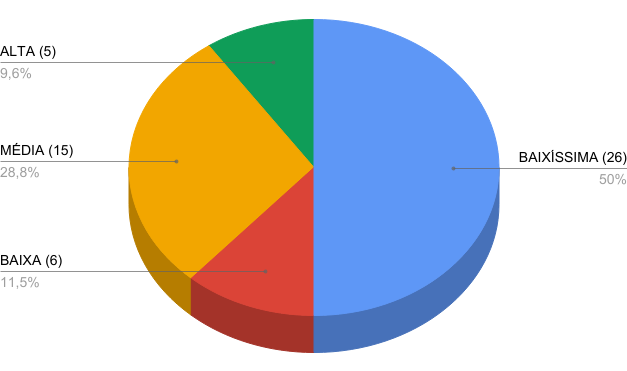
\includegraphics[width=0.45\textwidth]{grafico-recorrencia.png}
	\caption{Distribui\c{c}\~ao das Categorias x Recorr\^encia}
	\label{fig:CategoriaXRecorrencia}
\end{figure}


A Tabela \ref{tab:Categories} apresenta o n\'umero de ocorr\^encias das categorias de alta, m\'edia e baixa recorr\^encia em cada quest\~ao relacionada a boas e m\'as pr\'aticas. A \'ultima linha da tabela, \#Categorias, apresenta quantas categorias emergiram de cada quest\~ao, como cada quest\~ao est\'a diretamente ligada a um elemento do \textit{front-end} Android, podemos interpret\'a-la da seguinte forma: \textbf{quais s\~ao os pontos de aten\c{c}\~ao a serem analisados em determinado elemento Android?} A \'ultima coluna da tabela, \#Q, apresenta em quantas quest\~oes cada categoria surgiu, podemos interpret\'a-la da seguinte forma: \textbf{com base na categoria, quais elementos devem ser investigados}?

% Quando se criam categoriza\c{c}\~oes para auxiliar desenvolvedores a identificar pontos de aten\c{c}\~ao a serem avaliados e onde este pontos devem ser investigados especificamente no c\'odigo, pensando em qualidade de c\'odigo d\'a-se o nome de \textit{smells}. Portanto, nesta se\c{c}\~ao iremos compilar este conjunto de Android \textit{code smells} que identificamos atrav\'es das categoriza\c{c}\~oes.


\begin{table*}[t]
\centering
\footnotesize
\begin{tabular}{@{}p{3.8cm}p{0.3cm}p{.2cm}p{.2cm}p{.2cm}p{.2cm}p{.2cm}p{.2cm}p{.2cm}p{.2cm}p{.2cm}p{.4cm}p{.4cm}p{.4cm}p{.4cm}p{.4cm}p{.4cm}p{.4cm}p{.4cm}p{.4cm}p{0.2cm}@{}}
\toprule
\textbf{Categoria} & \multicolumn{1}{c}{\textbf{\#T}} & Q1 & Q2 & Q3 & Q4 & Q5 & Q6 & Q7 & Q8 & Q9 & Q10 & Q11 & Q12 & Q13 & Q14 & Q15 & Q16 & Q17 & Q18 &  \multicolumn{1}{c}{\textbf{\#Q}} \\
\hline
\multicolumn{2}{c}{\scriptsize{\textbf{ALTA RECORR\^ENCIA}}} \\
L\'ogica em Views							& \multicolumn{1}{c}{53} 	& \multicolumn{1}{c}{12} 	& \multicolumn{1}{c}{15} 	& \multicolumn{1}{c}{6} 	& \multicolumn{1}{c}{8} 	& \multicolumn{1}{c}{3} 	& \multicolumn{1}{c}{8} 	& \multicolumn{1}{c}{--} 	& \multicolumn{1}{c}{1} 	& \multicolumn{1}{c}{--} 	& \multicolumn{1}{c}{--} 	& \multicolumn{1}{c}{--} 	& \multicolumn{1}{c}{--} 	& \multicolumn{1}{c}{--} 	& \multicolumn{1}{c}{--} 	& \multicolumn{1}{c}{--} 	& \multicolumn{1}{c}{--} 	& \multicolumn{1}{c}{--} 	& \multicolumn{1}{c}{--} 	& \multicolumn{1}{c}{7} \\	
Padr\~ao de Nome de Recursos				& \multicolumn{1}{c}{24} 	& \multicolumn{1}{c}{1} 	& \multicolumn{1}{c}{--} 	& \multicolumn{1}{c}{--} 	& \multicolumn{1}{c}{--} 	& \multicolumn{1}{c}{--} 	& \multicolumn{1}{c}{--} 	& \multicolumn{1}{c}{--} 	& \multicolumn{1}{c}{--} 	& \multicolumn{1}{c}{3} 	& \multicolumn{1}{c}{2} 	& \multicolumn{1}{c}{3} 	& \multicolumn{1}{c}{2} 	& \multicolumn{1}{c}{8} 	& \multicolumn{1}{c}{2} 	& \multicolumn{1}{c}{3} 	& \multicolumn{1}{c}{--} 	& \multicolumn{1}{c}{--} 	& \multicolumn{1}{c}{--} 	& \multicolumn{1}{c}{8} \\	
Recursos M\'agicos							& \multicolumn{1}{c}{23} 	& \multicolumn{1}{c}{--} 	& \multicolumn{1}{c}{--} 	& \multicolumn{1}{c}{--} 	& \multicolumn{1}{c}{--} 	& \multicolumn{1}{c}{--} 	& \multicolumn{1}{c}{--} 	& \multicolumn{1}{c}{--} 	& \multicolumn{1}{c}{--} 	& \multicolumn{1}{c}{4} 	& \multicolumn{1}{c}{2} 	& \multicolumn{1}{c}{1} 	& \multicolumn{1}{c}{1} 	& \multicolumn{1}{c}{9} 	& \multicolumn{1}{c}{6} 	& \multicolumn{1}{c}{--} 	& \multicolumn{1}{c}{--} 	& \multicolumn{1}{c}{--} 	& \multicolumn{1}{c}{--} 	& \multicolumn{1}{c}{6} \\	
Views Aninhados								& \multicolumn{1}{c}{21} 	& \multicolumn{1}{c}{--} 	& \multicolumn{1}{c}{--} 	& \multicolumn{1}{c}{--} 	& \multicolumn{1}{c}{--} 	& \multicolumn{1}{c}{1} 	& \multicolumn{1}{c}{--} 	& \multicolumn{1}{c}{--} 	& \multicolumn{1}{c}{--} 	& \multicolumn{1}{c}{9} 	& \multicolumn{1}{c}{9} 	& \multicolumn{1}{c}{--} 	& \multicolumn{1}{c}{--} 	& \multicolumn{1}{c}{--} 	& \multicolumn{1}{c}{--} 	& \multicolumn{1}{c}{--} 	& \multicolumn{1}{c}{--} 	& \multicolumn{1}{c}{1} 	& \multicolumn{1}{c}{1} 	& \multicolumn{1}{c}{5} \\	

\vspace{1sp} \\
\multicolumn{2}{@{}c}{\scriptsize{\textbf{M\'EDIA RECORR\^ENCIA}}} \\ 
Padr\~ao MVP								& \multicolumn{1}{c}{17} 	& \multicolumn{1}{c}{8} 	& \multicolumn{1}{c}{2} 	& \multicolumn{1}{c}{5} 	& \multicolumn{1}{c}{--} 	& \multicolumn{1}{c}{--} 	& \multicolumn{1}{c}{--} 	& \multicolumn{1}{c}{--} 	& \multicolumn{1}{c}{--} 	& \multicolumn{1}{c}{--} 	& \multicolumn{1}{c}{--} 	& \multicolumn{1}{c}{--} 	& \multicolumn{1}{c}{--} 	& \multicolumn{1}{c}{--} 	& \multicolumn{1}{c}{--} 	& \multicolumn{1}{c}{--} 	& \multicolumn{1}{c}{--} 	& \multicolumn{1}{c}{2} 	& \multicolumn{1}{c}{--} 	& \multicolumn{1}{c}{4} \\
Acoplamento Entre Views						& \multicolumn{1}{c}{18} 	& \multicolumn{1}{c}{--} 	& \multicolumn{1}{c}{2} 	& \multicolumn{1}{c}{4} 	& \multicolumn{1}{c}{6} 	& \multicolumn{1}{c}{--} 	& \multicolumn{1}{c}{3} 	& \multicolumn{1}{c}{1} 	& \multicolumn{1}{c}{2} 	& \multicolumn{1}{c}{--} 	& \multicolumn{1}{c}{--} 	& \multicolumn{1}{c}{--} 	& \multicolumn{1}{c}{--} 	& \multicolumn{1}{c}{--} 	& \multicolumn{1}{c}{--} 	& \multicolumn{1}{c}{--} 	& \multicolumn{1}{c}{--} 	& \multicolumn{1}{c}{--} 	& \multicolumn{1}{c}{--} 	& \multicolumn{1}{c}{6} \\
Ciclo de Vida								& \multicolumn{1}{c}{16} 	& \multicolumn{1}{c}{4} 	& \multicolumn{1}{c}{3} 	& \multicolumn{1}{c}{3} 	& \multicolumn{1}{c}{5} 	& \multicolumn{1}{c}{--} 	& \multicolumn{1}{c}{--} 	& \multicolumn{1}{c}{1} 	& \multicolumn{1}{c}{--} 	& \multicolumn{1}{c}{--} 	& \multicolumn{1}{c}{--} 	& \multicolumn{1}{c}{--} 	& \multicolumn{1}{c}{--} 	& \multicolumn{1}{c}{--} 	& \multicolumn{1}{c}{--} 	& \multicolumn{1}{c}{--} 	& \multicolumn{1}{c}{--} 	& \multicolumn{1}{c}{--} 	& \multicolumn{1}{c}{--} 	& \multicolumn{1}{c}{5} \\
Use Include									& \multicolumn{1}{c}{15} 	& \multicolumn{1}{c}{--} 	& \multicolumn{1}{c}{--} 	& \multicolumn{1}{c}{--} 	& \multicolumn{1}{c}{--} 	& \multicolumn{1}{c}{--} 	& \multicolumn{1}{c}{--} 	& \multicolumn{1}{c}{--} 	& \multicolumn{1}{c}{--} 	& \multicolumn{1}{c}{12} 	& \multicolumn{1}{c}{2} 	& \multicolumn{1}{c}{--} 	& \multicolumn{1}{c}{--} 	& \multicolumn{1}{c}{--} 	& \multicolumn{1}{c}{--} 	& \multicolumn{1}{c}{--} 	& \multicolumn{1}{c}{--} 	& \multicolumn{1}{c}{1} 	& \multicolumn{1}{c}{--} 	& \multicolumn{1}{c}{3} \\
Padr\~ao View Holder						& \multicolumn{1}{c}{14} 	& \multicolumn{1}{c}{--} 	& \multicolumn{1}{c}{--} 	& \multicolumn{1}{c}{--} 	& \multicolumn{1}{c}{--} 	& \multicolumn{1}{c}{12} 	& \multicolumn{1}{c}{2} 	& \multicolumn{1}{c}{--} 	& \multicolumn{1}{c}{--} 	& \multicolumn{1}{c}{--} 	& \multicolumn{1}{c}{--} 	& \multicolumn{1}{c}{--} 	& \multicolumn{1}{c}{--} 	& \multicolumn{1}{c}{--} 	& \multicolumn{1}{c}{--} 	& \multicolumn{1}{c}{--} 	& \multicolumn{1}{c}{--} 	& \multicolumn{1}{c}{--} 	& \multicolumn{1}{c}{--} 	& \multicolumn{1}{c}{2} \\
Tamanho de Imagens Importam					& \multicolumn{1}{c}{12} 	& \multicolumn{1}{c}{--} 	& \multicolumn{1}{c}{--} 	& \multicolumn{1}{c}{--} 	& \multicolumn{1}{c}{--} 	& \multicolumn{1}{c}{--} 	& \multicolumn{1}{c}{--} 	& \multicolumn{1}{c}{--} 	& \multicolumn{1}{c}{--} 	& \multicolumn{1}{c}{1} 	& \multicolumn{1}{c}{1} 	& \multicolumn{1}{c}{--} 	& \multicolumn{1}{c}{--} 	& \multicolumn{1}{c}{--} 	& \multicolumn{1}{c}{--} 	& \multicolumn{1}{c}{4} 	& \multicolumn{1}{c}{6} 	& \multicolumn{1}{c}{--} 	& \multicolumn{1}{c}{--} 	& \multicolumn{1}{c}{4} \\
Comportamento Suspeito						& \multicolumn{1}{c}{14} 	& \multicolumn{1}{c}{1} 	& \multicolumn{1}{c}{1} 	& \multicolumn{1}{c}{--} 	& \multicolumn{1}{c}{--} 	& \multicolumn{1}{c}{1} 	& \multicolumn{1}{c}{3} 	& \multicolumn{1}{c}{5} 	& \multicolumn{1}{c}{3} 	& \multicolumn{1}{c}{--} 	& \multicolumn{1}{c}{--} 	& \multicolumn{1}{c}{--} 	& \multicolumn{1}{c}{--} 	& \multicolumn{1}{c}{--} 	& \multicolumn{1}{c}{--} 	& \multicolumn{1}{c}{--} 	& \multicolumn{1}{c}{--} 	& \multicolumn{1}{c}{--} 	& \multicolumn{1}{c}{--} 	& \multicolumn{1}{c}{6} \\
Classe Deus/Longa*							& \multicolumn{1}{c}{11} 	& \multicolumn{1}{c}{1} 	& \multicolumn{1}{c}{4} 	& \multicolumn{1}{c}{1} 	& \multicolumn{1}{c}{2} 	& \multicolumn{1}{c}{--} 	& \multicolumn{1}{c}{1} 	& \multicolumn{1}{c}{--} 	& \multicolumn{1}{c}{1} 	& \multicolumn{1}{c}{--} 	& \multicolumn{1}{c}{--} 	& \multicolumn{1}{c}{--} 	& \multicolumn{1}{c}{1} 	& \multicolumn{1}{c}{--} 	& \multicolumn{1}{c}{--} 	& \multicolumn{1}{c}{--} 	& \multicolumn{1}{c}{--} 	& \multicolumn{1}{c}{--} 	& \multicolumn{1}{c}{--} 	& \multicolumn{1}{c}{7} \\
Use Fragment								& \multicolumn{1}{c}{11} 	& \multicolumn{1}{c}{3} 	& \multicolumn{1}{c}{2} 	& \multicolumn{1}{c}{5} 	& \multicolumn{1}{c}{1} 	& \multicolumn{1}{c}{--} 	& \multicolumn{1}{c}{--} 	& \multicolumn{1}{c}{--} 	& \multicolumn{1}{c}{--} 	& \multicolumn{1}{c}{--} 	& \multicolumn{1}{c}{--} 	& \multicolumn{1}{c}{--} 	& \multicolumn{1}{c}{--} 	& \multicolumn{1}{c}{--} 	& \multicolumn{1}{c}{--} 	& \multicolumn{1}{c}{--} 	& \multicolumn{1}{c}{--} 	& \multicolumn{1}{c}{--} 	& \multicolumn{1}{c}{--} 	& \multicolumn{1}{c}{4} \\
Use Imagens Vetoriais						& \multicolumn{1}{c}{11} 	& \multicolumn{1}{c}{--} 	& \multicolumn{1}{c}{--} 	& \multicolumn{1}{c}{--} 	& \multicolumn{1}{c}{--} 	& \multicolumn{1}{c}{--} 	& \multicolumn{1}{c}{--} 	& \multicolumn{1}{c}{--} 	& \multicolumn{1}{c}{--} 	& \multicolumn{1}{c}{--} 	& \multicolumn{1}{c}{--} 	& \multicolumn{1}{c}{--} 	& \multicolumn{1}{c}{--} 	& \multicolumn{1}{c}{--} 	& \multicolumn{1}{c}{--} 	& \multicolumn{1}{c}{11} 	& \multicolumn{1}{c}{--} 	& \multicolumn{1}{c}{--} 	& \multicolumn{1}{c}{--} 	& \multicolumn{1}{c}{1} \\
Fragment Apenas Se Necess\'ario				& \multicolumn{1}{c}{10} 	& \multicolumn{1}{c}{--} 	& \multicolumn{1}{c}{--} 	& \multicolumn{1}{c}{8} 	& \multicolumn{1}{c}{2} 	& \multicolumn{1}{c}{--} 	& \multicolumn{1}{c}{--} 	& \multicolumn{1}{c}{--} 	& \multicolumn{1}{c}{--} 	& \multicolumn{1}{c}{--} 	& \multicolumn{1}{c}{--} 	& \multicolumn{1}{c}{--} 	& \multicolumn{1}{c}{--} 	& \multicolumn{1}{c}{--} 	& \multicolumn{1}{c}{--} 	& \multicolumn{1}{c}{--} 	& \multicolumn{1}{c}{--} 	& \multicolumn{1}{c}{--} 	& \multicolumn{1}{c}{--} 	& \multicolumn{1}{c}{2} \\
Use Arquiteturas Conhecidas					& \multicolumn{1}{c}{9} 	& \multicolumn{1}{c}{--} 	& \multicolumn{1}{c}{--} 	& \multicolumn{1}{c}{1} 	& \multicolumn{1}{c}{--} 	& \multicolumn{1}{c}{2} 	& \multicolumn{1}{c}{--} 	& \multicolumn{1}{c}{--} 	& \multicolumn{1}{c}{--} 	& \multicolumn{1}{c}{--} 	& \multicolumn{1}{c}{--} 	& \multicolumn{1}{c}{--} 	& \multicolumn{1}{c}{--} 	& \multicolumn{1}{c}{--} 	& \multicolumn{1}{c}{--} 	& \multicolumn{1}{c}{--} 	& \multicolumn{1}{c}{--} 	& \multicolumn{1}{c}{5} 	& \multicolumn{1}{c}{1} 	& \multicolumn{1}{c}{4} \\
Recurso de Estilo Deus						& \multicolumn{1}{c}{8} 	& \multicolumn{1}{c}{--} 	& \multicolumn{1}{c}{--} 	& \multicolumn{1}{c}{--} 	& \multicolumn{1}{c}{--} 	& \multicolumn{1}{c}{--} 	& \multicolumn{1}{c}{--} 	& \multicolumn{1}{c}{--} 	& \multicolumn{1}{c}{--} 	& \multicolumn{1}{c}{--} 	& \multicolumn{1}{c}{--} 	& \multicolumn{1}{c}{5} 	& \multicolumn{1}{c}{3} 	& \multicolumn{1}{c}{--} 	& \multicolumn{1}{c}{--} 	& \multicolumn{1}{c}{--} 	& \multicolumn{1}{c}{--} 	& \multicolumn{1}{c}{--} 	& \multicolumn{1}{c}{--} 	& \multicolumn{1}{c}{2} \\
Recurso de Strings Bagun\c{c}ado			& \multicolumn{1}{c}{8} 	& \multicolumn{1}{c}{--} 	& \multicolumn{1}{c}{--} 	& \multicolumn{1}{c}{--} 	& \multicolumn{1}{c}{--} 	& \multicolumn{1}{c}{--} 	& \multicolumn{1}{c}{--} 	& \multicolumn{1}{c}{--} 	& \multicolumn{1}{c}{--} 	& \multicolumn{1}{c}{--} 	& \multicolumn{1}{c}{--} 	& \multicolumn{1}{c}{--} 	& \multicolumn{1}{c}{--} 	& \multicolumn{1}{c}{4} 	& \multicolumn{1}{c}{4} 	& \multicolumn{1}{c}{--} 	& \multicolumn{1}{c}{--} 	& \multicolumn{1}{c}{--} 	& \multicolumn{1}{c}{--} 	& \multicolumn{1}{c}{2} \\
Atributos de Estilos Duplicados				& \multicolumn{1}{c}{8} 	& \multicolumn{1}{c}{--} 	& \multicolumn{1}{c}{--} 	& \multicolumn{1}{c}{--} 	& \multicolumn{1}{c}{--} 	& \multicolumn{1}{c}{--} 	& \multicolumn{1}{c}{--} 	& \multicolumn{1}{c}{--} 	& \multicolumn{1}{c}{--} 	& \multicolumn{1}{c}{1} 	& \multicolumn{1}{c}{2} 	& \multicolumn{1}{c}{2} 	& \multicolumn{1}{c}{2} 	& \multicolumn{1}{c}{--} 	& \multicolumn{1}{c}{--} 	& \multicolumn{1}{c}{--} 	& \multicolumn{1}{c}{--} 	& \multicolumn{1}{c}{1} 	& \multicolumn{1}{c}{--} 	& \multicolumn{1}{c}{5} \\

\vspace*{1sp} \\
\multicolumn{2}{@{}c}{\scriptsize{\textbf{BAIXA RECORR\^ENCIA}}} \\
Activity Inexistente  						& \multicolumn{1}{c}{7} 	& \multicolumn{1}{c}{2} 	& \multicolumn{1}{c}{4} 	& \multicolumn{1}{c}{--} 	& \multicolumn{1}{c}{--} 	& \multicolumn{1}{c}{--} 	& \multicolumn{1}{c}{--} 	& \multicolumn{1}{c}{--} 	& \multicolumn{1}{c}{1} 	& \multicolumn{1}{c}{--} 	& \multicolumn{1}{c}{--} 	& \multicolumn{1}{c}{--} 	& \multicolumn{1}{c}{--} 	& \multicolumn{1}{c}{--} 	& \multicolumn{1}{c}{--} 	& \multicolumn{1}{c}{--} 	& \multicolumn{1}{c}{--} 	& \multicolumn{1}{c}{--} 	& \multicolumn{1}{c}{--} 	& \multicolumn{1}{c}{3} \\
Ferramenta de DI							& \multicolumn{1}{c}{7} 	& \multicolumn{1}{c}{1} 	& \multicolumn{1}{c}{1} 	& \multicolumn{1}{c}{--} 	& \multicolumn{1}{c}{--} 	& \multicolumn{1}{c}{--} 	& \multicolumn{1}{c}{--} 	& \multicolumn{1}{c}{4} 	& \multicolumn{1}{c}{--} 	& \multicolumn{1}{c}{--} 	& \multicolumn{1}{c}{--} 	& \multicolumn{1}{c}{--} 	& \multicolumn{1}{c}{--} 	& \multicolumn{1}{c}{--} 	& \multicolumn{1}{c}{--} 	& \multicolumn{1}{c}{--} 	& \multicolumn{1}{c}{--} 	& \multicolumn{1}{c}{1} 	& \multicolumn{1}{c}{--} 	& \multicolumn{1}{c}{4} \\
Evite Imagens								& \multicolumn{1}{c}{7} 	& \multicolumn{1}{c}{--} 	& \multicolumn{1}{c}{--} 	& \multicolumn{1}{c}{--} 	& \multicolumn{1}{c}{--} 	& \multicolumn{1}{c}{--} 	& \multicolumn{1}{c}{--} 	& \multicolumn{1}{c}{--} 	& \multicolumn{1}{c}{--} 	& \multicolumn{1}{c}{1} 	& \multicolumn{1}{c}{--} 	& \multicolumn{1}{c}{--} 	& \multicolumn{1}{c}{--} 	& \multicolumn{1}{c}{--} 	& \multicolumn{1}{c}{--} 	& \multicolumn{1}{c}{4} 	& \multicolumn{1}{c}{2} 	& \multicolumn{1}{c}{--} 	& \multicolumn{1}{c}{--} 	& \multicolumn{1}{c}{3} \\
Reuso Excessivo de Strings					& \multicolumn{1}{c}{6} 	& \multicolumn{1}{c}{--} 	& \multicolumn{1}{c}{--} 	& \multicolumn{1}{c}{--} 	& \multicolumn{1}{c}{--} 	& \multicolumn{1}{c}{--} 	& \multicolumn{1}{c}{--} 	& \multicolumn{1}{c}{--} 	& \multicolumn{1}{c}{--} 	& \multicolumn{1}{c}{--} 	& \multicolumn{1}{c}{--} 	& \multicolumn{1}{c}{--} 	& \multicolumn{1}{c}{--} 	& \multicolumn{1}{c}{2} 	& \multicolumn{1}{c}{4} 	& \multicolumn{1}{c}{--} 	& \multicolumn{1}{c}{--} 	& \multicolumn{1}{c}{--} 	& \multicolumn{1}{c}{--} 	& \multicolumn{1}{c}{2} \\
Adapter Flex\'ivel							& \multicolumn{1}{c}{6} 	& \multicolumn{1}{c}{--} 	& \multicolumn{1}{c}{--} 	& \multicolumn{1}{c}{--} 	& \multicolumn{1}{c}{--} 	& \multicolumn{1}{c}{3} 	& \multicolumn{1}{c}{2} 	& \multicolumn{1}{c}{--} 	& \multicolumn{1}{c}{--} 	& \multicolumn{1}{c}{--} 	& \multicolumn{1}{c}{1} 	& \multicolumn{1}{c}{--} 	& \multicolumn{1}{c}{--} 	& \multicolumn{1}{c}{--} 	& \multicolumn{1}{c}{--} 	& \multicolumn{1}{c}{--} 	& \multicolumn{1}{c}{--} 	& \multicolumn{1}{c}{--} 	& \multicolumn{1}{c}{--} 	& \multicolumn{1}{c}{3} \\
Heran\c{c}a**								& \multicolumn{1}{c}{5} 	& \multicolumn{1}{c}{2} 	& \multicolumn{1}{c}{--} 	& \multicolumn{1}{c}{2} 	& \multicolumn{1}{c}{--} 	& \multicolumn{1}{c}{1} 	& \multicolumn{1}{c}{--} 	& \multicolumn{1}{c}{--} 	& \multicolumn{1}{c}{--} 	& \multicolumn{1}{c}{--} 	& \multicolumn{1}{c}{--} 	& \multicolumn{1}{c}{--} 	& \multicolumn{1}{c}{--} 	& \multicolumn{1}{c}{--} 	& \multicolumn{1}{c}{--} 	& \multicolumn{1}{c}{--} 	& \multicolumn{1}{c}{--} 	& \multicolumn{1}{c}{--} 	& \multicolumn{1}{c}{--} 	& \multicolumn{1}{c}{3} \\
Listener Escondido							& \multicolumn{1}{c}{3} 	& \multicolumn{1}{c}{--} 	& \multicolumn{1}{c}{--} 	& \multicolumn{1}{c}{--} 	& \multicolumn{1}{c}{--} 	& \multicolumn{1}{c}{--} 	& \multicolumn{1}{c}{--} 	& \multicolumn{1}{c}{--} 	& \multicolumn{1}{c}{3} 	& \multicolumn{1}{c}{--} 	& \multicolumn{1}{c}{--} 	& \multicolumn{1}{c}{--} 	& \multicolumn{1}{c}{--} 	& \multicolumn{1}{c}{--} 	& \multicolumn{1}{c}{--} 	& \multicolumn{1}{c}{--} 	& \multicolumn{1}{c}{--} 	& \multicolumn{1}{c}{--} 	& \multicolumn{1}{c}{--} 	& \multicolumn{1}{c}{1} \\
Opera\c{c}\~oes de IO							& \multicolumn{1}{c}{6} 	& \multicolumn{1}{c}{--} 	& \multicolumn{1}{c}{3} 	& \multicolumn{1}{c}{--} 	& \multicolumn{1}{c}{2} 	& \multicolumn{1}{c}{--} 	& \multicolumn{1}{c}{1} 	& \multicolumn{1}{c}{--} 	& \multicolumn{1}{c}{--} 	& \multicolumn{1}{c}{--} 	& \multicolumn{1}{c}{--} 	& \multicolumn{1}{c}{--} 	& \multicolumn{1}{c}{--} 	& \multicolumn{1}{c}{--} 	& \multicolumn{1}{c}{--} 	& \multicolumn{1}{c}{--} 	& \multicolumn{1}{c}{--} 	& \multicolumn{1}{c}{--} 	& \multicolumn{1}{c}{--} 	& \multicolumn{1}{c}{3} \\
\hline
\multicolumn{2}{r}{\textbf{\#Totais}}		& \multicolumn{1}{c}{35} 	& \multicolumn{1}{c}{37} 	& \multicolumn{1}{c}{35} 	& \multicolumn{1}{c}{26} 	& \multicolumn{1}{c}{23} 	& \multicolumn{1}{c}{20} 	& \multicolumn{1}{c}{11} 	& \multicolumn{1}{c}{11} 	& \multicolumn{1}{c}{31} 	& \multicolumn{1}{c}{19} 	& \multicolumn{1}{c}{11} 	& \multicolumn{1}{c}{9} 	& \multicolumn{1}{c}{23} 	& \multicolumn{1}{c}{16} 	& \multicolumn{1}{c}{22} 	& \multicolumn{1}{c}{8} 	& \multicolumn{1}{c}{11} 	& \multicolumn{1}{c}{2} \\
\hline
\multicolumn{2}{r}{\textbf{\#Categorias}}	& \multicolumn{1}{c}{10} 	& \multicolumn{1}{c}{10} 	& \multicolumn{1}{c}{9} 	& \multicolumn{1}{c}{7} 	& \multicolumn{1}{c}{7} 	& \multicolumn{1}{c}{7} 	& \multicolumn{1}{c}{4} 	& \multicolumn{1}{c}{6} 	& \multicolumn{1}{c}{7} 	& \multicolumn{1}{c}{7} 	& \multicolumn{1}{c}{4} 	& \multicolumn{1}{c}{5} 	& \multicolumn{1}{c}{4} 	& \multicolumn{1}{c}{4} 	& \multicolumn{1}{c}{4} 	& \multicolumn{1}{c}{2} 	& \multicolumn{1}{c}{6} 	& \multicolumn{1}{c}{2} \\
\hline
% \multicolumn{20}{@{}l@{}}{* Classe Deus \cite{Riel} e Classe Longa \cite{RefactoringFowler1999} s\~ao \textit{code smells} tradicionais previamente definidos em literaturas. ** Heran\c{c}a \'e um conceito da Programa\c{c}\~ao Orientada a Objetos \cite{WikipediaInhiritance}. \textbf{\#T}: recorr\^encia geral da categoria. \textbf{\#Q}: total de quest\~oes distintas em cada categoria. A linha \textbf{\#Totais}: total de respostas obtidas em cada quest\~ao. \textbf{\#Categorias}: total de categorias distinstas de cada quest\~ao.} \\

\multicolumn{20}{@{}l}{* Classe Deus \cite{Riel} e Classe Longa \cite{RefactoringFowler1999} s\~ao cheiros de c\'odigo tradicionais previamente definidos em literaturas.} \\
\multicolumn{20}{@{}l}{** Heran\c{c}a \'e um conceito da Programa\c{c}\~ao Orientada a Objetos \cite{WikipediaInhiritance}.} \\
\multicolumn{20}{@{}l}{Coluna \textbf{\#T}: recorr\^encia geral da categoria.} \\
\multicolumn{20}{@{}l}{Coluna \textbf{\#Q}: total de quest\~oes distintas em cada categoria.} \\
\multicolumn{20}{@{}l}{Linha \textbf{\#Totais}: total de respostas obtidas em cada quest\~ao.} \\
\multicolumn{20}{@{}l}{Linha \textbf{\#Categorias}: total de categorias distinstas de cada quest\~ao.} \\
\toprule
\end{tabular}
\caption{Lista de categorias de alta, m\'edia e baixa recorr\^encia.}
\label{tab:Categories}
\end{table*}


Esta se\c{c}\~ao est\'a organizada em 4 subse\c{c}\~oes, respectivamente abordando sobre as categorias de alta, m\'edia, baixa e baix\'issima recorr\^encia. A quantidade de respostas recebida por cada categoria \'e apresentada em detalhes na Tabela \ref{tab:Categories}.

\subsection{Categorias de Alta Recorr\^encia}
Obtivemos 4 categorias consideradas de alta recorr\^encia: L\'ogica em Views, Padr\~ao de Nome de Recursos, Recursos M\'agicos e Views Aninhados.


% \begin{table*}[t]
% \centering
% \caption{Lista de categorias de alta recorr\^encia.}
% \footnotesize
% \begin{tabular}{@{}p{2.9cm}p{1cm}|p{0.3cm}p{0.3cm}p{0.3cm}p{0.3cm}p{0.3cm}p{0.3cm}p{0.3cm}p{0.3cm}p{0.4cm}p{0.4cm}p{0.4cm}p{0.4cm}p{0.4cm}p{0.4cm}p{0.4cm}p{0.4cm}|p{1.5cm}@{}}
% \toprule
% \textbf{Categoria}	& \textbf{\#Total} 	& Q1 	& Q2 	& Q3 	& Q4 	& Q5 	& Q6 	& Q8 	& Q9 	& Q10 	& Q11 	& Q12 	& Q13 	& Q14 	& Q15 	& Q17 	& Q18 	&  \textbf{\#Quest\~oes} \\
% \hline
% No Logic In View				& 	\multicolumn{1}{c|}{53} 	& \multicolumn{1}{c}{12} 	& \multicolumn{1}{c}{15} 	& \multicolumn{1}{c}{6} 	& \multicolumn{1}{c}{8} 	& \multicolumn{1}{c}{3} 	& \multicolumn{1}{c}{8} 	& \multicolumn{1}{c}{1} 	& \multicolumn{1}{c}{--} 	& \multicolumn{1}{c}{--} 	& \multicolumn{1}{c}{--} 	& \multicolumn{1}{c}{--} 	& \multicolumn{1}{c}{--} 	& \multicolumn{1}{c}{--} 	& \multicolumn{1}{c}{--} 	& \multicolumn{1}{c}{--} 	& \multicolumn{1}{c|}{0} 	& \multicolumn{1}{c}{7}	\\
% Resource Name Pattern			& 	\multicolumn{1}{c|}{24} 	& \multicolumn{1}{c}{1} 	& \multicolumn{1}{c}{--} 	& \multicolumn{1}{c}{--} 	& \multicolumn{1}{c}{--} 	& \multicolumn{1}{c}{--} 	& \multicolumn{1}{c}{--} 	& \multicolumn{1}{c}{--} 	& \multicolumn{1}{c}{3} 	& \multicolumn{1}{c}{2} 	& \multicolumn{1}{c}{3} 	& \multicolumn{1}{c}{2} 	& \multicolumn{1}{c}{8} 	& \multicolumn{1}{c}{2} 	& \multicolumn{1}{c}{3} 	& \multicolumn{1}{c}{--} 	& \multicolumn{1}{c|}{0} 	& \multicolumn{1}{c}{8}	\\
% Magic Resource					& 	\multicolumn{1}{c|}{23} 	& \multicolumn{1}{c}{--} 	& \multicolumn{1}{c}{--} 	& \multicolumn{1}{c}{--} 	& \multicolumn{1}{c}{--} 	& \multicolumn{1}{c}{--} 	& \multicolumn{1}{c}{--} 	& \multicolumn{1}{c}{--} 	& \multicolumn{1}{c}{4} 	& \multicolumn{1}{c}{2} 	& \multicolumn{1}{c}{1} 	& \multicolumn{1}{c}{1} 	& \multicolumn{1}{c}{9} 	& \multicolumn{1}{c}{6} 	& \multicolumn{1}{c}{--} 	& \multicolumn{1}{c}{--} 	& \multicolumn{1}{c|}{0} 	& \multicolumn{1}{c}{6}	\\
% Nested Layout					& 	\multicolumn{1}{c|}{21} 	& \multicolumn{1}{c}{--} 	& \multicolumn{1}{c}{--} 	& \multicolumn{1}{c}{--} 	& \multicolumn{1}{c}{--} 	& \multicolumn{1}{c}{1} 	& \multicolumn{1}{c}{--} 	& \multicolumn{1}{c}{--} 	& \multicolumn{1}{c}{9} 	& \multicolumn{1}{c}{9} 	& \multicolumn{1}{c}{--} 	& \multicolumn{1}{c}{--} 	& \multicolumn{1}{c}{--} 	& \multicolumn{1}{c}{--} 	& \multicolumn{1}{c}{--} 	& \multicolumn{1}{c}{1} 	& \multicolumn{1}{c|}{1} 	& \multicolumn{1}{c}{5}	\\
% % \hline
% % \multicolumn{2}{r}{\textbf{\#Total}}										& \multicolumn{1}{c}{13} 	& \multicolumn{1}{c}{15} 	& \multicolumn{1}{c}{6} 	& \multicolumn{1}{c}{8} 	& \multicolumn{1}{c}{4} 	& \multicolumn{1}{c}{8} 	& \multicolumn{1}{c}{1} 	& \multicolumn{1}{c}{16} 	& \multicolumn{1}{c}{13} 	& \multicolumn{1}{c}{4} 	& \multicolumn{1}{c}{3} 	& \multicolumn{1}{c}{17} 	& \multicolumn{1}{c}{8} 	& \multicolumn{1}{c}{3} 	& \multicolumn{1}{c}{1} 	& \multicolumn{1}{c}{1} 	& \\
% \hline
% \multicolumn{19}{@{}l}{\scriptsize{* As categorias de alta recorr\^encia n\~ao n\~ao receberam respostas \`as quest\~oes Q7 e Q16.}} \\
% \toprule
% \end{tabular}
% \label{tab:CategoriasAltaRecorrencia}
% \end{table*}

\subsubsection{L\'ogica em Views}
Esta categoria re\'une respostas que indicam como m\'a pr\'atica haver regra de neg\'ocio nos elementos Android afetados. De forma similar, respostas indicam como boas pr\'aticas n\~ao haver c\'odigo de regra de neg\'ocio. Exemplos de frases que indicaram m\'as pr\'aticas s\~ao: P16 sobre \textsc{Activitys} diz \textit{``Fazer l\'ogica de neg\'ocio''} (tradu\c{c}\~ao livre), P19 diz \textit{``Colocar regra de neg\'ocio no adapter''} e P11 diz \textit{``Manter l\'ogica de neg\'ocio em Fragments''} (tradu\c{c}\~ao livre). Exemplos de frases que indicaram boas pr\'atica s\~ao: P16 diz sobre \textsc{Activitys} \textit{``Elas representam uma \'unica tela e apenas interagem com a UI, qualquer l\'ogica deve ser delegada para outra classe''} (tradu\c{c}\~ao livre), P23 diz \textit{``Apenas c\'odigo relacionado \`a Interface de Usu\'ario nas Activities''}, P40 diz \textit{``Adapters devem apenas se preocupar sobre como mostrar os dados, sem trabalh\'a-los''}. Os elementos que entraram nessa categoria foram: \textsc{Activitys}, \textsc{Fragments}, \textsc{Listeners} e \textsc{Adapters}. 


\subsubsection{Padr\~ao de Nome de Recursos}
Esta categoria re\'une respostas que indicam como m\'a pr\'atica o n\~ao uso de um padr\~ao de nomenclatura a ser usado nos recursos da aplica\c{c}\~ao. De forma similar, respostas indicam como boas pr\'aticas o uso de um padr\~ao de nomenclatura a ser usados nos recursos. Exemplos de frases que indicaram m\'as pr\'aticas s\~ao: P8 sobre \textsc{Style Resources} diz \textit{``[...] o nome das strings sem um contexto''} (tradu\c{c}\~ao livre), P37 tamb\'em sobre \textsc{Style Resources} diz \textit{``Nada al\'em de ter uma boa conven\c{c}\~ao de nomes''} (tradu\c{c}\~ao livre), ainda P37, por\'em sobre \textsc{Layout Resources} diz \textit{``Mantenha uma conven\c{c}\~ao de nomes da sua escolha [...]''} (tradu\c{c}\~ao livre). Exemplos de frases que indicaram boas pr\'atica s\~ao: P27 diz sobre \textsc{String Resources} \textit{``Iniciar o nome de uma string com o nome da tela onde vai ser usada''}, P43 sobre \textsc{Layout Resources} diz \textit{``Ter uma boa conven\c{c}\~ao de nomea\c{c}\~ao''} (tradu\c{c}\~ao livre), P11 diz sobre \textsc{Style Resources} \textit{``[...] colocar um bom nome [...]''} (tradu\c{c}\~ao livre). Os elementos que entraram nessa categoria foram: \textsc{Activitys}, \textsc{Layout Resources}, \textsc{String Resources}, \textsc{Style Resources} e \textsc{Drawable Resources}. 

Dentre as respostas, algumas indicaram padr\~oes de prefer\^encia. P11 indica usar prefixos nos \textsc{Layout Resources}: \texttt{activity\_}, \texttt{fragment\_}, \texttt{ui\_} (para UI customizadas). P12 sugeriu usar sufixos em \textsc{Activitys}: \texttt{\_Activity}. Os padr\~oes indicados para \textsc{String Resources} foram: P27 indicou \textit{``Iniciar o nome da string com o nome da tela onde vai ser usada''}, P6 sugeriu a conven\c{c}\~ao \texttt{[screen]\_[type]\_[text]} e citou como exemplo \texttt{welcome\_message\_title}. P34 indicou que deve-se usar como prefixo o recurso usando a string, por exemplo \texttt{dialog.STRING\_NAME} ou \texttt{hint.STRING\_NAME}. De forma similar por\'em sem sugerir um exemplo, P4 sugeriu basear o nome da string no nome do recurso que a esta usando. N\~ao foram sugeridos nenhum padr\~ao para \textsc{Styles Resources} e \textsc{Drawable Resources}.

\subsubsection{Recursos M\'agicos}
Esta categoria re\'une respostas que indicam como m\'a pr\'atica o uso direto de valores como, por exemplo, strings, n\'umeros e cores, sem a cria\c{c}\~ao um recurso. De forma similar, respostas indicam como boas pr\'aticas o uso de um padr\~ao de nomenclatura a ser usados nos recursos. O nome dessa categoria foi inspirado no cheiro de c\'odigo \textit{Magic Number} \cite{Martin:2008:CCH:1388398} que trata sobre n\'umeros usados diretamente no c\'odigo. Exemplos de frases que indicaram m\'as pr\'aticas s\~ao: P23 diz \textit{``Strings diretamente no c\'odigo''}, P31 e P35 falam respectivamente sobre n\~ao extrair as strings e sobre n\~ao extrair os valores dos arquivos de layout. Exemplos de frases que indicaram boas pr\'atica s\~ao: P7 diz \textit{``Sempre pegar valores de string ou dp de seus respectivos resources para facilitar''}, P36 diz para \textit{``sempre adicionar as strings em resources para traduzir em diversos idiomas [...]''}. Os elementos que entraram nessa categoria foram: \textsc{Layout Resources}, \textsc{String Resources} e \textsc{Style Resources}. 

\subsubsection{Views Aninhados} 
Esta categoria re\'une respostas que indicam como m\'a pr\'atica o uso de profundos aninhamentos na constru\c{c}\~ao de layouts. De forma similar, respostas indicam como boas pr\'aticas evitar ao m\'aximo o aninhamento de \textit{views}. Exemplos de frases que indicaram m\'as pr\'aticas s\~ao: P26 diz \textit{``Hierarquia de views longas''} (tradu\c{c}\~ao livre), P4 aborda a mesma ideia ao dizer \textit{``Estruturas profundamente aninhadas''} (tradu\c{c}\~ao livre), P39 diz \textit{``Hierarquias desnecess\'arias''} e P45 diz \textit{``Criar muitos ViewGroups dentro de ViewGroups''}. Exemplos de frases que indicaram boas pr\'atica s\~ao: P4 diz \textit{``tento usar o m\'inimo de layout aninhado''}, P19 diz \textit{``Utilizar o m\'inimo de camadas poss\'ivel''}, P8 diz \textit{``[...] n\~ao fazer uma hierarquia profunda de ViewGroups [...]''}. Apenas o elemento \textsc{Layout Resources} recebeu esta categoria. O site oficial do Android conta com informa\c{c}\~oes e ferramentas automatizadas para lidar com esse sintoma \cite{OptmizingViewHierarchies}. 

\subsection{Categorias de M\'edia Recorr\^encia}
Obtivemos 16 categorias consideradas de m\'edia recorr\^encia: Acoplamento Entre Views, Padr\~ao MVP, Ciclo de Vida, Use Include, Padr\~ao View Holder, Comportamento Suspeito, Tamanho de Imagens Importam, Classe Deus/Longa, Use Fragment, Use Imagens Vetoriais, Fragment Apenas Se Necess\'ario, Use Arquiteturas Conhecidas, Recurso de Estilo Deus, Recurso de Strings Bagun\c{c}ado e Atributos de Estilos Duplicados.


\subsubsection{Acoplamento Entre Views}
Esta categoria re\'une respostas que indicam como m\'a pr\'atica o acoplamento entre \textsc{Activitys}, \textsc{Fragments}, \textsc{Adapters} e \textsc{Listeners}, ou seja, a exist\^encia de refer\^encias diretas entre elas. De forma similar, respostas indicam como boas pr\'aticas que estas classes n\~ao se conhe\c{c}am diretamente. Com base nas respostas, identificamos 3 situa\c{c}\~oes onde essa m\'a pr\'atica \'e percebida.

O primeira situa\c{c}\~ao \'e quando o \textsc{Fragment} est\'a acoplado \`a \textsc{Activitys}, outros \textsc{Fragments} ou componentes. Sobre o acoplamento de \textsc{Fragments} com \textsc{Activitys}, P19 diz \textit{``Acoplar o fragment a activity ao inv\'es de utilizar interfaces \'e uma pr\'atica ruim''}. P10, P31 e P45 indicam como m\'a pr\'atica \textit{``acoplar o \textsc{Fragment} com a \textsc{Activity}''} (tradu\c{c}\~ao livre). Sobre o acoplamento de \textsc{Fragments} com outros \textsc{Fragments}, P37 diz que \textit{``Fragments nunca devem tentar falar uns com os outros diretamente''} e P45 diz \textit{``[\'e uma m\'a pr\'atica] integragir com outro Fragment diretamente''} (tradu\c{c}\~ao livre). Sobre o \textsc{Fragments} serem acoplados a outros componentes, P6 diz \textit{``Seja um componente de UI reutiliz\'avel. Ent\~ao evite depend\^encia de outros componentes da aplica\c{c}\~ao''}. Como boa pr\'atica, para a comunica\c{c}\~ao entre essas classes, s\~ao indicados: o uso de \textit{interfaces}, o m\'etodo \textsc{onAttach} existente em \textsc{Fragments} (este m\'etodo \'e disparado pelo Android ao associar um \textsc{Fragment} a uma \textsc{Activity}) ou a biblioteca \textit{EventBus} \cite{EventBusAndroid}. P36 diz \textit{``Criar uma interface para a comunica\c{c}\~ao entre Activity e Fragment, ou utilizar o EventBus.''} e P44 diz \textit{``Use e abuse do m\'etodo onAttach para se comunicar com Activity''}. 

A segunda situa\c{c}\~ao \'e quando o \textsc{Listener} est\'a acoplado \`a \textsc{Activitys}. P40 diz que \'e uma m\'a pr\'atica \textit{``[o \textsc{Listener}] conter uma refer\^encia forte \`a Activitys''} (tradu\c{c}\~ao livre), P4 exprime a mesma ideia com uma frase um pouco diferente. 

A terceira situa\c{c}\~ao \'e quando o \textsc{Adapter} est\'a acoplado \`a \textsc{Activitys} ou \textsc{Fragments}. P10 indicou como m\'a pr\'atica em \textit{Adapters} o \textit{``alto acoplamento com a Activity''} e P45 exprime a mesma ideia ao dizer \textit{``Acessar Activitys ou Fragments diretamente''}. 

Os elementos que entraram nessa categoria foram: \textsc{Activitys}, \textsc{Fragments}, \textsc{Listeners} e \textsc{Adapters}. 


\subsubsection{Padr\~ao MVP}
Esta categoria re\'une respostas que indicam como m\'a pr\'atica -----------. De forma similar, respostas indicam como boas pr\'aticas --------. Exemplos de frases que indicaram m\'as pr\'aticas s\~ao: ---------. Exemplos de frases que indicaram boas pr\'atica s\~ao: --------------------. Os elementos que entraram nessa categoria foram: ---------------. 

\subsubsection{Ciclo de Vida}
Esta categoria re\'une respostas que indicam como m\'a pr\'atica -----------. De forma similar, respostas indicam como boas pr\'aticas --------. Exemplos de frases que indicaram m\'as pr\'aticas s\~ao: ---------. Exemplos de frases que indicaram boas pr\'atica s\~ao: --------------------. Os elementos que entraram nessa categoria foram: ---------------. 

\subsubsection{Use Include}
Esta categoria re\'une respostas que indicam como m\'a pr\'atica -----------. De forma similar, respostas indicam como boas pr\'aticas --------. Exemplos de frases que indicaram m\'as pr\'aticas s\~ao: ---------. Exemplos de frases que indicaram boas pr\'atica s\~ao: --------------------. Os elementos que entraram nessa categoria foram: ---------------. 

\subsubsection{Padr\~ao View Holder}
Esta categoria re\'une respostas que indicam como m\'a pr\'atica -----------. De forma similar, respostas indicam como boas pr\'aticas --------. Exemplos de frases que indicaram m\'as pr\'aticas s\~ao: ---------. Exemplos de frases que indicaram boas pr\'atica s\~ao: --------------------. Os elementos que entraram nessa categoria foram: ---------------. 

\subsubsection{Comportamento Suspeito}
Esta categoria re\'une respostas que indicam como m\'a pr\'atica -----------. De forma similar, respostas indicam como boas pr\'aticas --------. Exemplos de frases que indicaram m\'as pr\'aticas s\~ao: ---------. Exemplos de frases que indicaram boas pr\'atica s\~ao: --------------------. Os elementos que entraram nessa categoria foram: ---------------. 

\subsubsection{Tamanho de Imagens Importam}
Esta categoria re\'une respostas que indicam como m\'a pr\'atica -----------. De forma similar, respostas indicam como boas pr\'aticas --------. Exemplos de frases que indicaram m\'as pr\'aticas s\~ao: ---------. Exemplos de frases que indicaram boas pr\'atica s\~ao: --------------------. Os elementos que entraram nessa categoria foram: ---------------. 

\subsubsection{Classe Deus/Longa}
Esta categoria re\'une respostas que indicam como m\'a pr\'atica -----------. De forma similar, respostas indicam como boas pr\'aticas --------. Exemplos de frases que indicaram m\'as pr\'aticas s\~ao: ---------. Exemplos de frases que indicaram boas pr\'atica s\~ao: --------------------. Os elementos que entraram nessa categoria foram: ---------------. 

\subsubsection{Use Fragment}
Esta categoria re\'une respostas que indicam como m\'a pr\'atica -----------. De forma similar, respostas indicam como boas pr\'aticas --------. Exemplos de frases que indicaram m\'as pr\'aticas s\~ao: ---------. Exemplos de frases que indicaram boas pr\'atica s\~ao: --------------------. Os elementos que entraram nessa categoria foram: ---------------. 

\subsubsection{Use Imagens Vetoriais}
Esta categoria re\'une respostas que indicam como m\'a pr\'atica -----------. De forma similar, respostas indicam como boas pr\'aticas --------. Exemplos de frases que indicaram m\'as pr\'aticas s\~ao: ---------. Exemplos de frases que indicaram boas pr\'atica s\~ao: --------------------. Os elementos que entraram nessa categoria foram: ---------------. 

\subsubsection{Fragment Apenas Se Necess\'ario}
Esta categoria re\'une respostas que indicam como m\'a pr\'atica -----------. De forma similar, respostas indicam como boas pr\'aticas --------. Exemplos de frases que indicaram m\'as pr\'aticas s\~ao: ---------. Exemplos de frases que indicaram boas pr\'atica s\~ao: --------------------. Os elementos que entraram nessa categoria foram: ---------------. 

\subsubsection{Use Arquiteturas Conhecidas}
Esta categoria re\'une respostas que indicam como m\'a pr\'atica -----------. De forma similar, respostas indicam como boas pr\'aticas --------. Exemplos de frases que indicaram m\'as pr\'aticas s\~ao: ---------. Exemplos de frases que indicaram boas pr\'atica s\~ao: --------------------. Os elementos que entraram nessa categoria foram: ---------------. 

\subsubsection{Recurso de Estilo Deus}
Esta categoria re\'une respostas que indicam como m\'a pr\'atica -----------. De forma similar, respostas indicam como boas pr\'aticas --------. Exemplos de frases que indicaram m\'as pr\'aticas s\~ao: ---------. Exemplos de frases que indicaram boas pr\'atica s\~ao: --------------------. Os elementos que entraram nessa categoria foram: ---------------. 

\subsubsection{Recurso de Strings Bagun\c{c}ado}
Esta categoria re\'une respostas que indicam como m\'a pr\'atica -----------. De forma similar, respostas indicam como boas pr\'aticas --------. Exemplos de frases que indicaram m\'as pr\'aticas s\~ao: ---------. Exemplos de frases que indicaram boas pr\'atica s\~ao: --------------------. Os elementos que entraram nessa categoria foram: ---------------. 

\subsubsection{Atributos de Estilos Duplicados}
Esta categoria re\'une respostas que indicam como m\'a pr\'atica -----------. De forma similar, respostas indicam como boas pr\'aticas --------. Exemplos de frases que indicaram m\'as pr\'aticas s\~ao: ---------. Exemplos de frases que indicaram boas pr\'atica s\~ao: --------------------. Os elementos que entraram nessa categoria foram: ---------------. 




\subsection{Categorias de Baixa Recorr\^encia}
Obtivemos 8 categorias consideradas de baixa recorr\^encia: Evite Imagens, Activity Inexistente, Ferramenta de DI, Reuso Excessivo de Strings, Adapter Flex\'ivel, Opera\c{c}\~oes de IO, Heran\c{c}a e Listener Escondido.

\subsubsection{Evite Imagens}
Esta categoria re\'une respostas que indicam como m\'a pr\'atica -----------. De forma similar, respostas indicam como boas pr\'aticas --------. Exemplos de frases que indicaram m\'as pr\'aticas s\~ao: ---------. Exemplos de frases que indicaram boas pr\'atica s\~ao: --------------------. Os elementos que entraram nessa categoria foram: ---------------. 


\subsubsection{Activity Inexistente}
Esta categoria re\'une respostas que indicam como m\'a pr\'atica -----------. De forma similar, respostas indicam como boas pr\'aticas --------. Exemplos de frases que indicaram m\'as pr\'aticas s\~ao: ---------. Exemplos de frases que indicaram boas pr\'atica s\~ao: --------------------. Os elementos que entraram nessa categoria foram: ---------------. 


\subsubsection{Ferramenta de DI}
Esta categoria re\'une respostas que indicam como m\'a pr\'atica -----------. De forma similar, respostas indicam como boas pr\'aticas --------. Exemplos de frases que indicaram m\'as pr\'aticas s\~ao: ---------. Exemplos de frases que indicaram boas pr\'atica s\~ao: --------------------. Os elementos que entraram nessa categoria foram: ---------------. 


\subsubsection{Reuso Excessivo de Strings}
Esta categoria re\'une respostas que indicam como m\'a pr\'atica -----------. De forma similar, respostas indicam como boas pr\'aticas --------. Exemplos de frases que indicaram m\'as pr\'aticas s\~ao: ---------. Exemplos de frases que indicaram boas pr\'atica s\~ao: --------------------. Os elementos que entraram nessa categoria foram: ---------------. 


\subsubsection{Adapter Flex\'ivel}
Esta categoria re\'une respostas que indicam como m\'a pr\'atica -----------. De forma similar, respostas indicam como boas pr\'aticas --------. Exemplos de frases que indicaram m\'as pr\'aticas s\~ao: ---------. Exemplos de frases que indicaram boas pr\'atica s\~ao: --------------------. Os elementos que entraram nessa categoria foram: ---------------. 


\subsubsection{Opera\c{c}\~oes de IO}
Esta categoria re\'une respostas que indicam como m\'a pr\'atica -----------. De forma similar, respostas indicam como boas pr\'aticas --------. Exemplos de frases que indicaram m\'as pr\'aticas s\~ao: ---------. Exemplos de frases que indicaram boas pr\'atica s\~ao: --------------------. Os elementos que entraram nessa categoria foram: ---------------. 


\subsubsection{Heran\c{c}a}
Esta categoria re\'une respostas que indicam como m\'a pr\'atica -----------. De forma similar, respostas indicam como boas pr\'aticas --------. Exemplos de frases que indicaram m\'as pr\'aticas s\~ao: ---------. Exemplos de frases que indicaram boas pr\'atica s\~ao: --------------------. Os elementos que entraram nessa categoria foram: ---------------. 


\subsubsection{Listener Escondido}
Esta categoria re\'une respostas que indicam como m\'a pr\'atica -----------. De forma similar, respostas indicam como boas pr\'aticas --------. Exemplos de frases que indicaram m\'as pr\'aticas s\~ao: ---------. Exemplos de frases que indicaram boas pr\'atica s\~ao: --------------------. Os elementos que entraram nessa categoria foram: ---------------. 



% \subsection{Categorias de Baix\'issima Recorr\^encia}
% Obtivemos 29 categorias consideradas de baix\'issima recorr\^encia: MVC, Clean Architecture, Don't Use Fragment, Nested Fragment, Mix String Resources With Business Logic, Use 9 Patch Files, Dealing With App Stack Manually, Styles Knows Too Much, Package Structure, MVVM, Activity Handle More Than One Layout, Bad Relative, Deprecated Attributes, Fat onCreate, HTML Into String File, Inherit From Support Library Always, Listener Has A Valid Context, Safe Adapter, Single Activity, Static Things On Adapter, Style Into String File, Use Constraint Layout, Dead Resources, DRY, SOLID, Reuse, Singleton, Opened Activity e Unnecessary ViewGroup









\section{Discussion}
% -*- root: article.tex -*-
% \lettrine[nindent=0em,lines=2]{L}

[Under construction] \\

% Consideramos inconclusivo se a utliza\c{c}\~ao de Fragments \'e recomendada ou n\~ao. 2 participantes afirmaram enfaticamente que n\~ao se deve usar \textsc{Fragments}, por exemplo, segundo P7, uma m\'a pr\'atica sobre \textsc{Fragments} \'e ``o uso deles''.


%----------------------------------------------------------------------------------------
%	REFERENCE LIST
%----------------------------------------------------------------------------------------

\bibliographystyle{plain}
\bibliography{bibliograph}


\end{document}
